
\begin{Large}
\begin{center}
\textbf{CUESTIONARIO LABORATORIO N 5} \\
\end{center}
\end{Large}

\section{Los valores introducidos al archivo sysctl.conf ¿que representan?} 


\begin{itemize}

\item fs.suiddumpable:\\
Esto controla si el núcleo puede ser volcado desde un programa seguid como se describe anteriormente. Vea abajo. Este es un sintonizador de kernel. a idea es que, si hay volcados de memoria y un usuario regular puede leerlos, es posible que encuentren información privilegiada. Si el programa se descarga bien, tenía información privilegiada en la memoria, y el usuario puede leer el volcado, pueden encontrar esa información privilegiada.\\\\

\item fs.aio-max-nr:\\
Define el máximo número de eventos permitidos en todos los contextos asíncronos de E/S. El valor predeterminado es 65536. Observe que al cambiar este valor no se preasigna o redimensiona ninguna estructura de datos de kernel.\\\\

\item fs.file-max:\\
Lista el número máximo de identificadores de archivos asignados por el kernel. El valor predeterminado coincide con el valor de files-stat.max-files en el kernel, el cual se establece al valor más grande, ya sea de (mempages * (PAGE-SIZE / 1024)) / 10, o NR-FILE (8192 en Red Hat Enterprise Linux). El aumento de este valor puede corregir errores ocasionados por la falta de identificadores de archivos disponibles.\\\\

\item kernel.shmmni:\\
Para hacer un cambio permanente, agregue la siguiente l´ınea al archivo /etc/sysctl.conf(su configuración puede variar). Este archivo se utiliza durante el proceso de arranque.\\\\

\item kernel.sem:\\
256 tamaño de la RAM en GB\\\\

\item net.ipv4.ip-local-port-range:\\
En Linux, hay un para ‘metro sysctl llamado ip-local-port-rangeque define el puerto mínimo y máximo que una conexión de red puede usar como su puerto de origen (local). Esto se aplica a las conexiones TCP y UDP.\\\\

\item net.core.rmem-default:\\
Oracle recomienda que el tamaño predeterminado y máximo del búfer de envío ( SO-SNDBUF opción de socket) y el tamaño del búfer de recepción ( SO-RCVBUF opción de socket) se establezcan en 256 KB. TCP y UDP utilizan los buffers de recepción para retener los datos recibidos hasta que la aplicación los lea. El búfer de recepción no puede desbordarse porque el par no tiene permiso para enviar datos más allá´ de la ventana del tamaño del búfer. Esto significa que los datagramas se descartaran si no caben en el búfer de recepción de socket. Esto podría hacer que el remitente abrume al receptor.\\\\
\item net.core.rmem-max:\\
Esto establece el tamaño máximo del búfer de recepción del SO para todos los tipos de conexiones.\\\\
\item net.core.wmem-default:\\
Esto establece el tamaño predeterminado del búfer de recepción del sistema operativo para todos los tipos de conexiones.\\\\
\item net.core.wmem-max:\\
Esto establece el tamaño máximo del búfer de envío del sistema operativo para todos los tipos de conexiones.\\\\


\end{itemize} 

\section{¿Con que usuario(s) puedo conectarme al servidor a través del Administrador Empresarial?} 

\begin{itemize}
\item SYS:\\\\
Todas las tablas y vistas para el diccionario de datos de la base de datos están almacenados en el esquema SYS. Estas tablas y vistas son críticas para el funcionamiento de la base de datos ORACLE. Para mantener la integridad del diccionario de datos, las tablas del esquema SYS son manipulados solo por la base de datos. Nunca se debería modificar algo o crear tablas en el esquema del usuario SYS.\\\\

\item SYSTEM:\\\\
El usuario SYSTEM se utiliza para crear tablas y vistas adicionales que muestran información administrativa, tablas internas y vistas utilizado por varias opciones y herramientas de la base de datos ORACLE. No se recomienda utilizar el esquema SYSTEM para almacenar tablas de interés para usuarios no administrativos.\\\\

\\\
\end{itemize} 

\section{Capture una imagen de pantalla del navegador con el Administrador Empresarial, con el nombre de su servidor e iniciada la sesión del usuario SYS.}\\\\
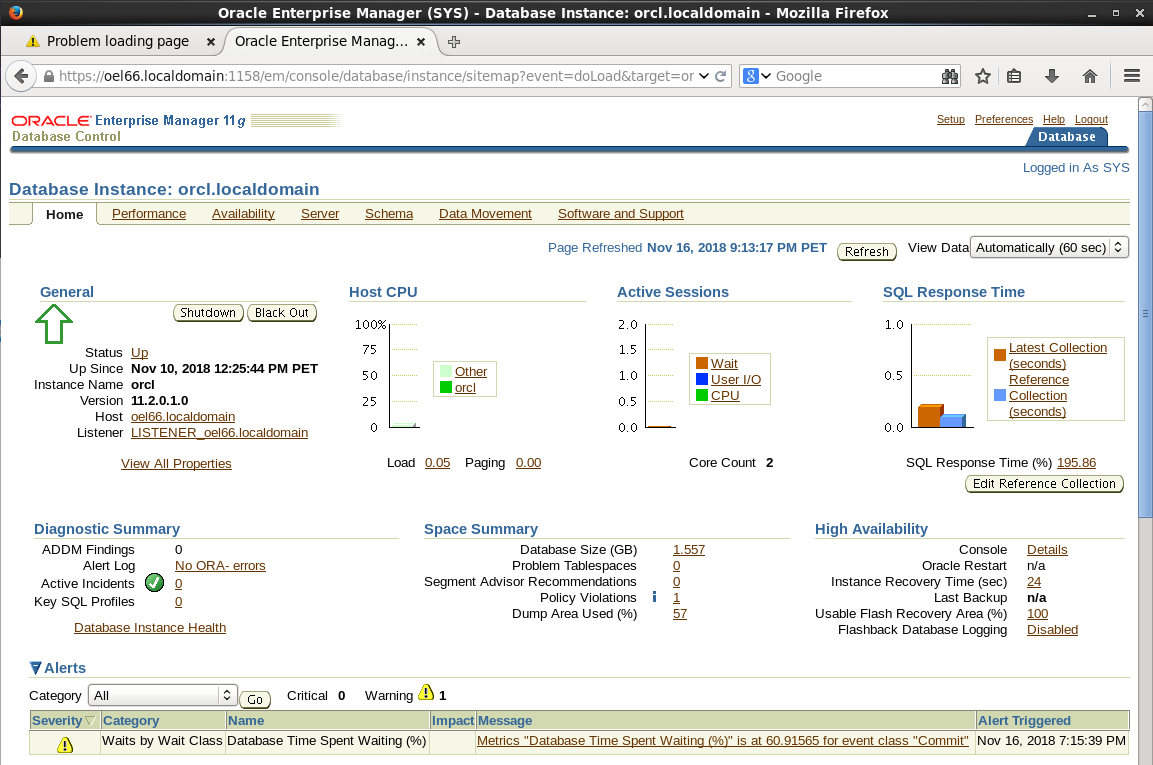
\includegraphics[width=18cm]{./Imagenes/usuariosys}


